\begin{frame}{Solución}
La principal contribución es el desarrollo de una
heurística para acelerar la ejecución del
algoritmo K-means para grandes colecciones de datos
de alta dimensionalidad.

\begin{itemize}
\item Dado un conjunto de centroides, evitar el calculo
de distancia entre vectores, tomados por pares, para obtener una 
partición de la colección. Los autores proponen una 
una asignación basada en el vecino más cercano de cada centroide.

\item Evitar el cálculo costoso de el verdadero centroide de 
cada cluster. Proponen una heurística para elegir el centroide
de una manera eficiente.
\end{itemize} 
\end{frame}

\begin{frame}{Heurísticas para el particionamiento rápido}

El principal cuello de botella del algoritmo K-means está
en la asignación de cada vector no centroide $d\in D - \cup_{k=1}^K$
a un cluster. Esto se logra eficientemente con la ayuda de la estructura
de datos \textbf{lista invertida}.

La lista invertida es particularmente adecuada para calcular
eficientemente el conjunto $TOP(x)$ para un vector dado $x$.
$TOP(x)$ nos da una lista de los vectores más similares
con respecto al vector actual $x$.

El algoritmo propuesto, al que llaman \textbf{FPAC} (Fast PArtitional
Clustering), utiliza la heurística de vecino más cercano, es decir,
$TOP(x)$ como operación fundamental.

\end{frame}


\begin{frame}{Inverted Index-Inverted List}
\begin{figure}
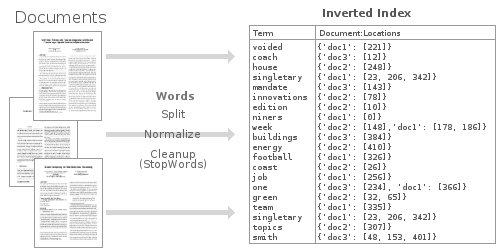
\includegraphics[scale=0.5]{img/invertedIndex}
\end{figure}
\end{frame}


\begin{frame}{Centroides como consultas}

Para asignar un cluster a un vector no centroide $d$, se
usan los $K$ centroides como consultas. El objetivo es encontrar el 
conjunto de los vectores más cercanos (más similares), $TOP(x)$,
para cada centroide $x$.
Si los centroides son diferentes entre ellos, es decir, no hay
similitud en el contenido tópico, se espera que las ranked lists
obtenidas de cada centroide, denotadas por $L(C_k)$,
tengan una intersección pequeña.

Si un vector $d$  se obtiene del conjunto $TOP$ de sólo
una ranked list $L(C_k)$, se incluye en el conjunto de vectores
asignados al cluster correspondiente a $C_k$.


Si un vector $d$ se encuentra en múltiples ranked lists, se asigna
al cluster cuyo score normalizado de similitud es el máximo.

\end{frame}


\begin{frame}{Formulación de las consultas y recuperación}

El algoritmo FPAC 

\end{frame}